\chapter{GUI}
\label{gui}

\section{Overview}

The following environment is required:

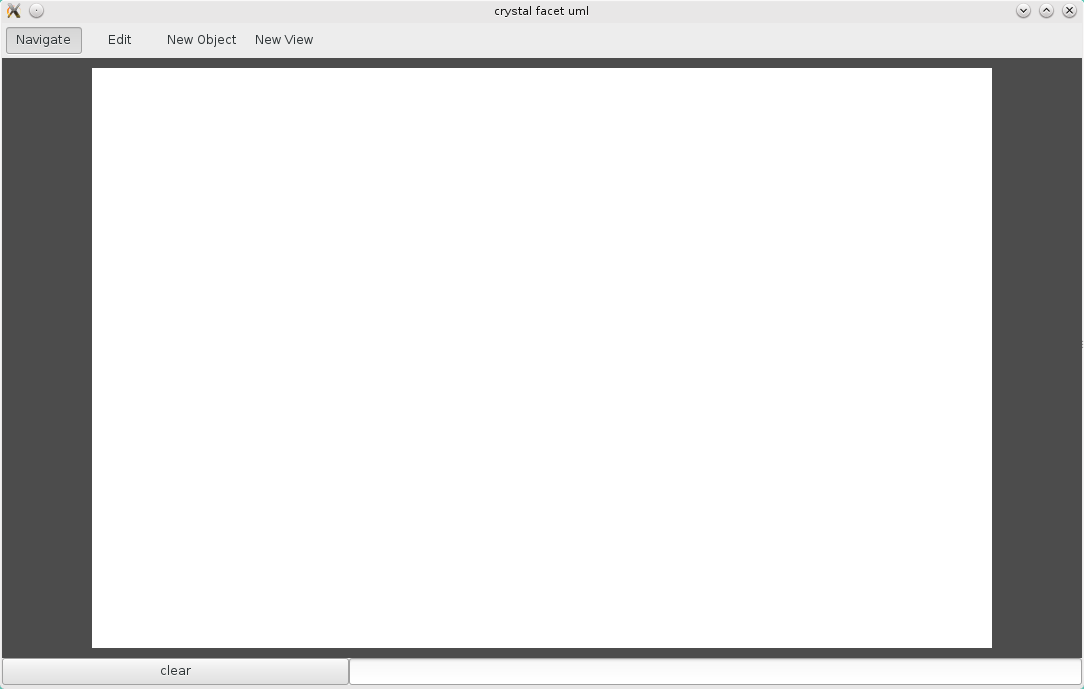
\includegraphics[width=10cm]{screenshot_1.png}


\includegraphics[width=10cm]{../../gui/source/resources/crystal_facet_uml.pdf}


crystal\_facet\_uml is a uml diagram drawing tool
that creates a set of consistent uml diagrams.

If started in graphical mode, it shows a window with
\begin{itemize}
\item toolbar on top,
\item drawing area in the center,
\item element configuration widgets below and
\item an optional notification bar at the bottom.
\end{itemize}

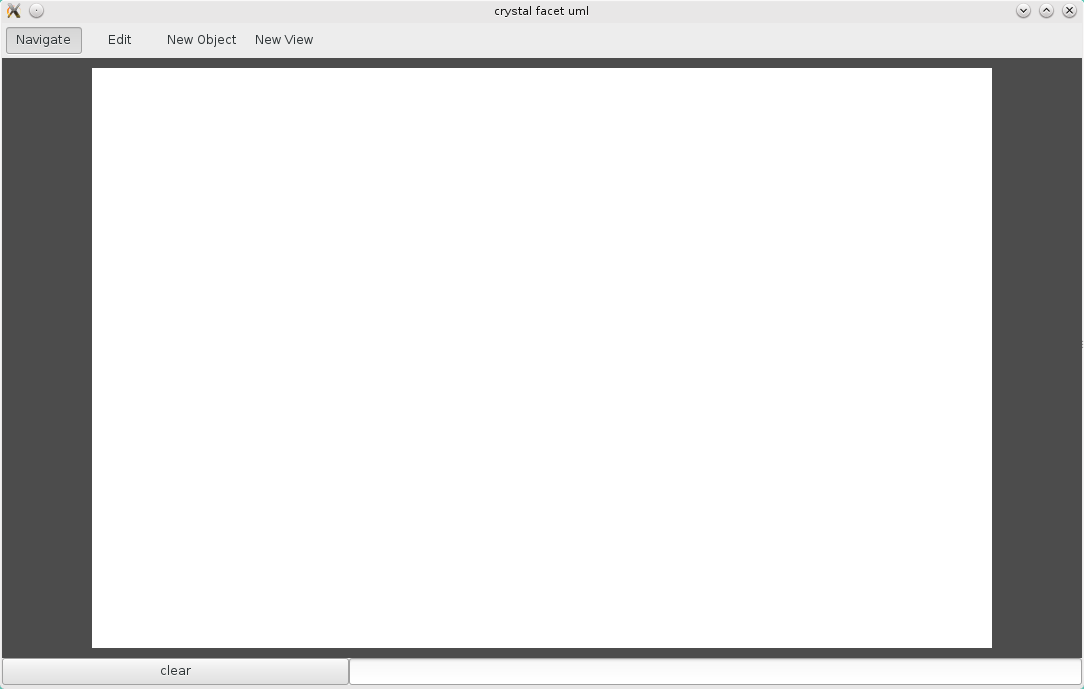
\includegraphics[width=10cm]{screenshot_1.png}

Additionally, crystal\_facet\_uml can be started from command line
to check and repair database files.
Run
code{.sh}
./crystal\_facet\_uml -h
endcode
to get a list of supported parameters.

\section{Tool Bar}

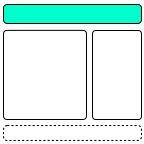
\includegraphics[width=10cm]{main_window_sketch_1.png}

\subsection{Create/Use DB}


\includegraphics[width=10cm]{../../gui/source/resources/file_use_db.pdf}
\begin{itemize}
\item Opens an existing database file or creates a new database file
\end{itemize}

\subsection{Export}


\includegraphics[width=10cm]{../../gui/source/resources/file_export.pdf}
\begin{itemize}
\item Exports all diagrams to the selected folder (supported formats are txt, png, pdf, ps and svg)
\end{itemize}

\subsection{New Window}


\includegraphics[width=10cm]{../../gui/source/resources/file_new_window.pdf}
\begin{itemize}
\item Opens another window on the same database.
\end{itemize}

\subsection{Navigate}


\includegraphics[width=10cm]{../../gui/source/resources/tool_navigate.pdf}
\begin{itemize}
\item Navigate to parent or child diagrams
\item Create a new diagram
\end{itemize}

\subsection{Edit}


\includegraphics[width=10cm]{../../gui/source/resources/tool_edit.pdf}
\begin{itemize}
\item Modify elements in the diagram
\end{itemize}

\subsection{Create}


\includegraphics[width=10cm]{../../gui/source/resources/tool_create.pdf}
\begin{itemize}
\item Create elements in the diagram
\end{itemize}

\subsection{Cut}


\includegraphics[width=10cm]{../../gui/source/resources/edit_cut.pdf}
\begin{itemize}
\item Cut all pink-cornered elements to the clipboard (features of classifiers are cut independantly of their corner-colors)
\end{itemize}

\subsection{Copy}


\includegraphics[width=10cm]{../../gui/source/resources/edit_copy.pdf}
\begin{itemize}
\item Copy all pink-cornered elements to the clipboard (features of classifiers are copied independantly of their corner-colors)
\end{itemize}

\subsection{Paste}


\includegraphics[width=10cm]{../../gui/source/resources/edit_paste.pdf}
\begin{itemize}
\item Pastes diagrams and classifiers from the clipboard to the uml model. (Relationships are not pasted)
    If id and name are identical to an existing element, an instance of the existing element is pasted to the diagram.
    Otherwise a new element is created.
\end{itemize}

\subsection{Delete}


\includegraphics[width=10cm]{../../gui/source/resources/edit_delete.pdf}
\begin{itemize}
\item Deletes all pink-cornered elements. This operation may fail if marked elements have unmarked children.
\end{itemize}

\subsection{Instantiate}


\includegraphics[width=10cm]{../../gui/source/resources/edit_instantiate.pdf}
\begin{itemize}
\item Toggles the pink-cornered classifiers between classes and instances. (Does not work for relationships and features)
\end{itemize}

\subsection{Highlight}


\includegraphics[width=10cm]{../../gui/source/resources/edit_highlight.pdf}
\begin{itemize}
\item Toggles the pink-cornered classifiers between yellow-marked, greyed-out and normal. (Does not work for relationships and features)
\end{itemize}

\subsection{Reset Selection}


\includegraphics[width=10cm]{../../gui/source/resources/edit_reset.pdf}
\begin{itemize}
\item Resets the pink-cornered selection
\end{itemize}

\subsection{Undo}


\includegraphics[width=10cm]{../../gui/source/resources/edit_undo.pdf}
\begin{itemize}
\item Un-does the last operation (Opening a database and exporting files cannot be undone)
\end{itemize}

\subsection{Redo}


\includegraphics[width=10cm]{../../gui/source/resources/edit_redo.pdf}
\begin{itemize}
\item Re-does the last un-done operation
\end{itemize}

\subsection{About}


\includegraphics[width=10cm]{../../gui/source/resources/crystal_facet_uml.pdf}
\begin{itemize}
\item Shows version, license and copyrights
\end{itemize}

\section{Drawing Area}

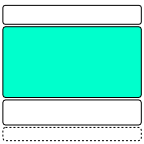
\includegraphics[width=10cm]{main_window_sketch_2.png}

Diagrams are layouted automatically. You can influence the locations of classifiers only.
When adding too many classifiers or relations, auto layouting may not achieve the expected results.
In many cases, splitting the diagram into two or more diagrams solves the layouting issues and
at the same time improves understandability by focusing on one aspect/topic per diagram.

\subsection{Navigate}


\includegraphics[width=10cm]{../../gui/source/resources/tool_navigate.pdf}
\begin{itemize}
\item To navigate to the parent diagram, click on the parent diagram.
\item To navigate to a child diagram, click on the child diagram.
\item To create a diagram, click on the + sign.
\item To restructure the diagram tree by shifting a child diagram up and the parent down, click on the child diagram and press F7.
\end{itemize}

\subsection{Edit}


\includegraphics[width=10cm]{../../gui/source/resources/tool_edit.pdf}
\begin{itemize}
\item To move classifiers within the diagram, press, drag and release the mouse button.
\item To select the diagram or a classifier or a feature or a relationship with yellow corners, click on this object.
\item To mark diagram and/or classifiers and/or features and/or relationships with pink corners, click on these objects twice.
\end{itemize}

\subsection{Create}


\includegraphics[width=10cm]{../../gui/source/resources/tool_create.pdf}
\begin{itemize}
\item To create a classifier, click at an empty space in the diagram.
\item To create a child classifier, click into the white space of a classifier.
    Alternatively, create a classifier and a containment relation.
\item To create a relationship, press on the source classifier and drag it to the destination classifier.
\item To create a feature, click onto a classifier (name or border).
\end{itemize}

\section{Element Configuration}

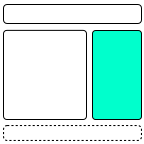
\includegraphics[width=10cm]{main_window_sketch_3.png}

Edit the properties of the yellow-cornered object.

\begin{itemize}
\item 0.: name of the focused object
\item 1.: stereotype/valuetype of the focused object (deactivated depending on object-type)
\item 2.: type of the focused object
\item 3.: description of the focused object
\end{itemize}

\subsection{Maximum stringlengths}

All strings (names, descriptions, stereotypes) have a maximum length.

Ascii characters require one, most other characters two bytes.
Current sizes in bytes are:

Classifiers:
\begin{itemize}
\item DATA\_CLASSIFIER\_MAX\_NAME\_LENGTH = 47,
\item DATA\_CLASSIFIER\_MAX\_STEREOTYPE\_LENGTH = 47,
\item DATA\_CLASSIFIER\_MAX\_DESCRIPTION\_LENGTH = 4095,
\end{itemize}

Features:
\begin{itemize}
\item DATA\_FEATURE\_MAX\_KEY\_LENGTH = 47,  (name)
\item DATA\_FEATURE\_MAX\_VALUE\_LENGTH = 255,  (type)
\item DATA\_FEATURE\_MAX\_DESCRIPTION\_LENGTH = 1023,
\end{itemize}

Relationships:
\begin{itemize}
\item DATA\_RELATIONSHIP\_MAX\_NAME\_LENGTH = 47,
\item DATA\_RELATIONSHIP\_MAX\_DESCRIPTION\_LENGTH = 1023,
\end{itemize}

Diagrams:
\begin{itemize}
\item DATA\_DIAGRAM\_MAX\_NAME\_LENGTH = 47,
\item DATA\_DIAGRAM\_MAX\_DESCRIPTION\_LENGTH = 8191,
\end{itemize}

\subsection{Commit}


\includegraphics[width=10cm]{../../gui/source/resources/edit_commit.pdf}
\begin{itemize}
\item Stores the latest changes to the database immediately. This feature is optional, it is not necessary to explicitly save the file.
\end{itemize}

\section{Notification Bar}


\includegraphics[height=10.5cm]{main_window_sketch_4.png}

\subsection{Information}


\includegraphics[width=10cm]{../../gui/source/resources/message_info.pdf}
\begin{itemize}
\item Informs on success of an operation, e.g. an export
\end{itemize}

\subsection{Warning}


\includegraphics[width=10cm]{../../gui/source/resources/message_warn.pdf}
\begin{itemize}
\item Informs on a possible problem
\end{itemize}

\subsection{Error}


\includegraphics[width=10cm]{../../gui/source/resources/message_error.pdf}
\begin{itemize}
\item Informs on an error
\end{itemize}

\section{Further Information}

\subsection cfu-dowload Download
Find the latest version at:
\begin{itemize}
\item https://sourceforge.net/projects/crystal-facet-uml/
\item https://github.com/awarnke/crystal\_facet\_uml
\item https://build.opensuse.org/package/show/home:awarnke/crystal\_facet\_uml
\end{itemize}

User documentation is available here:
\begin{itemize}
\item http://www.andreaswarnke.de/crystal\_facet\_uml/crystal\_facet\_uml\_user\_documentation.pdf
\item https://github.com/awarnke/crystal\_facet\_uml/blob/master/doxygen\_build/crystal\_facet\_uml\_user\_documentation.pdf
\end{itemize}

\subsection{License}
License of crystal\_facet\_uml is Apache-2.0.
crystal\_facet\_uml contains sqlite which is Public Domain.
Unit tests are based on embunit (MIT/X Consortium License).

(c) 2016-2018 A.Warnke; Email-contact: cfu-at-andreaswarnke-dot-de


